\section{Conclusioni e Risultati}
In questa sezione si confronteranno i risultati delle metriche menzionate nella sezione \ref{ssec: Criteria} e si faranno delle considerazioni finali.
\subsection{Analisi della Confusion Matrix}

Si può chiaramente notare come il modello K-NearestNeighbors con preprocessing predica discretamente bene le classi  "Many septa" e "Cyrrosis", ma faccia molta fatica a prevedere correttamente le prime due classi ovvero "Portal Fibrosis"  e "Few Septa". Mentre le altre varianti, Decision tree con preprocessing, senza preprocessing, e KNN senza preprocessing hanno una predizione molto scarsa su tutte e quattro le classi. (vedi fig. \ref{eq: confusion matrix}
\clearpage
\subsection{Performance per Modello}

Vengono riportate le metriche di prestazione di ciascun modello.

% Please add the following required packages to your document preamble:
% \usepackage{booktabs}
% \usepackage{multirow}
\begin{table}[ht]
\centering
\begin{tabular}{@{}lrcccc@{}}
\toprule
                                                                  & \multicolumn{1}{l}{}                                        & \multicolumn{4}{c}{\textbf{Average}}                                                                                                                                              \\ \midrule
\multicolumn{1}{|l|}{}                                            & \multicolumn{1}{l|}{}                                       & \multicolumn{1}{l|}{\textit{Precision}}    & \multicolumn{1}{r|}{\textit{Recall}}       & \multicolumn{1}{l|}{\textit{f1 score}}     & \multicolumn{1}{l|}{\textit{Accuracy}}     \\ \midrule
\multicolumn{1}{|l|}{\multirow{5}{*}{\textbf{For KNN}}}           & \multicolumn{1}{r|}{With Preprocessing}                     & \multicolumn{1}{c|}{0.30}                  & \multicolumn{1}{c|}{0.31}                  & \multicolumn{1}{c|}{0.27}                  & \multicolumn{1}{c|}{0.30}                  \\ \cmidrule(l){2-6} 
\multicolumn{1}{|l|}{}                                            & \multicolumn{1}{r|}{\multirow{3}{*}{Without Preprocessing}} & \multicolumn{1}{c|}{\multirow{3}{*}{0.27}} & \multicolumn{1}{c|}{\multirow{3}{*}{0.26}} & \multicolumn{1}{c|}{\multirow{3}{*}{0.26}} & \multicolumn{1}{c|}{\multirow{3}{*}{0.26}} \\
\multicolumn{1}{|l|}{}                                            & \multicolumn{1}{r|}{}                                       & \multicolumn{1}{c|}{}                      & \multicolumn{1}{c|}{}                      & \multicolumn{1}{c|}{}                      & \multicolumn{1}{c|}{}                      \\
\multicolumn{1}{|l|}{}                                            & \multicolumn{1}{r|}{}                                       & \multicolumn{1}{c|}{}                      & \multicolumn{1}{c|}{}                      & \multicolumn{1}{c|}{}                      & \multicolumn{1}{c|}{}                      \\ \cmidrule(l){2-6} 
\multicolumn{1}{|l|}{}                                            & \multicolumn{1}{r|}{Without Preprocessing, with CV}         & \multicolumn{1}{c|}{0.25}                  & \multicolumn{1}{c|}{0.25}                  & \multicolumn{1}{c|}{0.24}                  & \multicolumn{1}{c|}{0.25}                  \\ \midrule
                                                                  &                                                             &                                            &                                            &                                            &                                            \\ \midrule
\multicolumn{1}{|l|}{\multirow{5}{*}{\textbf{For Decision Tree}}} & \multicolumn{1}{r|}{With Preprocessing}                     & \multicolumn{1}{c|}{0.20}                  & \multicolumn{1}{c|}{0.26}                  & \multicolumn{1}{c|}{0.26}                  & \multicolumn{1}{c|}{0.26}                  \\ \cmidrule(l){2-6} 
\multicolumn{1}{|l|}{}                                            & \multicolumn{1}{r|}{\multirow{3}{*}{Without Preprocessing}} & \multicolumn{1}{c|}{\multirow{3}{*}{0.26}} & \multicolumn{1}{c|}{\multirow{3}{*}{0.26}} & \multicolumn{1}{c|}{\multirow{3}{*}{0.26}} & \multicolumn{1}{c|}{\multirow{3}{*}{0.26}} \\
\multicolumn{1}{|l|}{}                                            & \multicolumn{1}{r|}{}                                       & \multicolumn{1}{c|}{}                      & \multicolumn{1}{c|}{}                      & \multicolumn{1}{c|}{}                      & \multicolumn{1}{c|}{}                      \\
\multicolumn{1}{|l|}{}                                            & \multicolumn{1}{r|}{}                                       & \multicolumn{1}{c|}{}                      & \multicolumn{1}{c|}{}                      & \multicolumn{1}{c|}{}                      & \multicolumn{1}{c|}{}                      \\ \cmidrule(l){2-6} 
\multicolumn{1}{|l|}{}                                            & \multicolumn{1}{r|}{Without Preprocessing, with CV}         & \multicolumn{1}{c|}{0.25}                  & \multicolumn{1}{c|}{0.25}                  & \multicolumn{1}{c|}{0.24}                  & \multicolumn{1}{c|}{0.25}                  \\ \midrule
                                                                  & \multicolumn{1}{l}{}                                        &                                            & \multicolumn{1}{r}{}                       & \multicolumn{1}{l}{}                       & \multicolumn{1}{l}{}                       \\ \bottomrule
\end{tabular}

\caption{Performance e Confronto dei Modelli}
\label{tab:Performance_Modelli}
\end{table}
Si può notare chiaramente come il miglior classificatore sia il \textbf{KNN} con preprocessing e cross validation. 
L'accuracy migliore per il Decision Tree è quella utilizzando il preprocessing e cross validation. 
Il motivo per il quale si hanno metriche così basse è dovuto molto probabilemte alla complessità del problema trattato e il basso numero di samples del dataset (solo 1385). Sicuramente con un maggior numero di samples, quindi un numero maggiore di dati di nuovi pazienti soggetti all'epatite C, si otterrebbero significativi risultati.

\subsection{Ensemble}

Qui vengono mostrati i risultati dell'Ensemble sia del Decision Tree che del KNN con dati preprocessati, ovvero i due algoritmi con le migliori performance. I risultati sull'accuracy sono i seguenti:
\begin{itemize}
    \item Ensemble con Decision Tree: accuracy=0.2238. I parametri passati sono il numero di stimatori, settato a 100. Ovvero ci sono 100 Decision Tree che lavorano in parallelo. Purtroppo in questo caso l'accuracy è molto bassa, fin troppo.
    \item Ensemble con KNN: accuracy=0.288. I Paramentri passati anche qui sono il numero di stimatori, settato a 100. 
\end{itemize}

\subsection{ROC curve e Precision vs Recall curve}

   
\begin{figure}[H]
    \centering
    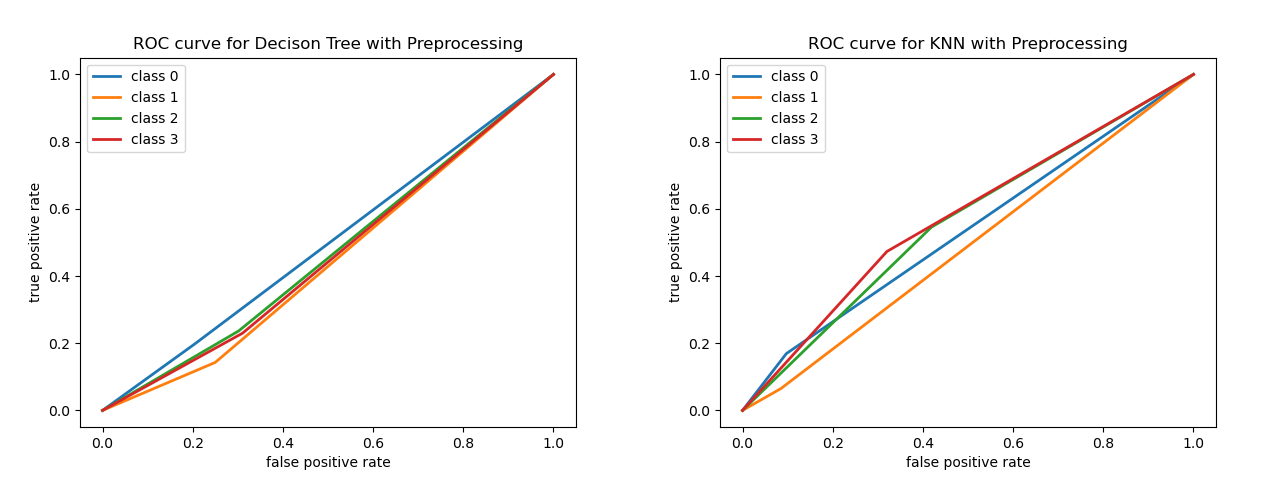
\includegraphics[width=1\columnwidth]{figures/ROC curve DT preprocROC KNN preproc.png}
    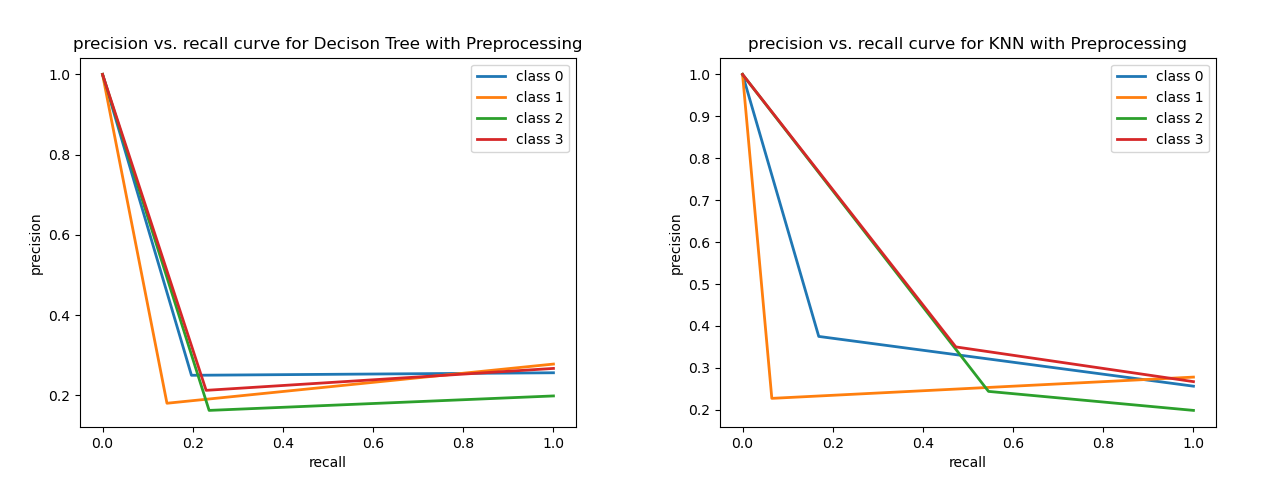
\includegraphics[width=1\columnwidth]{figures/DT Precision vs Recall PreprocPrecision vs Recall KNN preproc.png}
    \caption{ROC curves and Precision vs Recall curves}
    \label{fig:Roc curves}
\end{figure}

Si può osservare senza dubbio che le Roc curves hanno un andamento rappresentativo delle prestazioni riportate a tab. \ref{tab:Performance_Modelli}. Infatti una ROC curve che partendo dall'origine arriva alle coordinate (1,1) indicherebbe che il classificatore è perfetto, ovvero predice in modo esatto le classi. In realtà le immagini sopra mostrate, indicano il contrario per quanto riguarda sopratutto il Decision tree. Infatti la prima classe, la 0, ovvero quella corrispondente alla Portal fibrosis, viene rappresentata con una retta con pendenza a 45 gradi. Ciò significa che il classificatore diventa un classificatore casuale. Al contempo nella ROC curve del KNN sembra esserci un buon risultato di predizione, anche se la classe 1, ovvero "few septa", sembra essere predetta anch'essa casualmente.
Questo tipo di osservazione, si può fare attraverso anche un'altra metrica, chiamata \textbf{AUC}, ovvero Area Under the Curve. Quest'area è proprio l'area sottesa alla curva ROC, il cui valore è compreso tra 0 e 1. Come evidenziato prima, una retta che parte dall'origine (0,0) e finisce nel "top-right corner" (1,1) di questo grafico, avrà come area sottesa 0.5. Tale valore corrisponde appunto ad un classificatore casuale.
\clearpage
\subsection{Prestazioni}
Vengono riportati anche i tempi di processing dei modelli con e senza preprocessing.
\begin{table}[ht]
\centering
\begin{tabular}{@{}lcccll@{}}
\toprule
 & \multicolumn{1}{l}{}                                        & \multicolumn{4}{c}{\textbf{}}                                         \\ \midrule
\multicolumn{1}{|l|}{}                                            & \multicolumn{1}{c|}{}                                       & \multicolumn{4}{c|}{\textit{Processing Time (secs)}}                  \\ \midrule
\multicolumn{1}{|l|}{\multirow{4}{*}{\textbf{For KNN}}}           & \multicolumn{1}{c|}{With Preprocessing}                     & \multicolumn{4}{c|}{0.01197}                                          \\ \cmidrule(l){2-6} 
\multicolumn{1}{|l|}{}                                            & \multicolumn{1}{c|}{\multirow{3}{*}{Without Preprocessing}} & \multicolumn{4}{c|}{\multirow{3}{*}{0.016998}}                        \\
\multicolumn{1}{|l|}{}                                            & \multicolumn{1}{c|}{}                                       & \multicolumn{4}{c|}{}                                                 \\
\multicolumn{1}{|l|}{}                                            & \multicolumn{1}{c|}{}                                       & \multicolumn{4}{c|}{}                                                 \\ \midrule
                                                                  &                                                             &  &                      & \multicolumn{1}{c}{} & \multicolumn{1}{c}{} \\ \midrule
\multicolumn{1}{|l|}{\multirow{5}{*}{\textbf{For Decision Tree}}} & \multicolumn{1}{c|}{With Preprocessing}                     & \multicolumn{4}{c|}{0.00090}                                          \\ \cmidrule(l){2-6} 
\multicolumn{1}{|l|}{}                                            & \multicolumn{1}{c|}{\multirow{3}{*}{Without Preprocessing}} & \multicolumn{4}{c|}{\multirow{3}{*}{0.00200}}                         \\
\multicolumn{1}{|l|}{}                                            & \multicolumn{1}{c|}{}                                       & \multicolumn{4}{c|}{}                                                 \\
\multicolumn{1}{|l|}{}                                            & \multicolumn{1}{c|}{}                                       & \multicolumn{4}{c|}{}                                                 \\ \cmidrule(l){2-6} 
\multicolumn{1}{|l|}{}                                            & \multicolumn{5}{r|}{}                                                                                                               \\ \midrule
                                                                  & \multicolumn{1}{l}{}                                        &  & \multicolumn{1}{r}{} &                      &                      \\ \bottomrule
\end{tabular}
\end{table}
\newline Si nota chiaramente come gli algoritmi, con il preprocessing, e quindi con minor numero di dati tramite la features selection, ci impieghino sensibilmente meno a predire il risultato. 

